\documentclass[xcolor=dvipsnames]{beamer}

\usetheme{Darmstadt}
\usefonttheme[onlylarge]{structurebold}
\setbeamerfont*{frametitle}{size=\normalsize,series=\bfseries}
\setbeamertemplate{navigation symbols}{}

\usepackage[english]{babel}
\usepackage[cp1250]{inputenc}
\usepackage{times}
\usepackage[T1]{fontenc}


\usepackage{graphicx,amsmath} % Add all your packages here
\usepackage{amsfonts}
%\usepackage{listings}


\usepackage{url}

\usepackage{tikz}
\usetikzlibrary{arrows}
\tikzstyle{block}=[draw opacity=0.7,line width=1.4cm]


% correct bad hyphenation here
\hyphenation{op-tical net-works semi-conduc-tor IEEEtran}


\title{Towards Semantic Annotation Supported by Dependency Linguistics and ILP}

\author[D�dek]
{Jan D�dek}

\institute[MFF UK]
{
Department of Software Engineering, Faculty of Mathematics and Physics, Charles University in Prague, Czech Republic
}

\date[SAIAW WI 2009]
{ISWC 2010, Nov 9, 2010, Shanghai, China\\Doctoral Consortium}



\begin{document}

\begin{frame}
  \titlepage
\end{frame}

\begin{frame}{Outline}
  \tableofcontents
\end{frame}


\section{Introduction}

\subsection{Motivation}

\begin{frame}{Motivation}
\begin{enumerate}
	\item The goal of the Semantic Web evolution
	\begin{itemize}
		\item Bring structure to unstructured resources
	\end{itemize}
	\bigskip
	\item Complex linguistic tools
	\begin{itemize}
		\item The challenge of machine understanding of text  
	\end{itemize}
\end{enumerate}
\rule{0.8\hsize}{1pt}
\medskip
\begin{itemize}
	\item Using linguistics and Information Extraction for the Semantic Web
	\begin{itemize}
		\item Semantic annotation
	\end{itemize}
\end{itemize}
\end{frame}




\subsection{Linguistics we have used}

\begin{frame}{Layers of linguistic annotation in PDT}
\begin{columns}
\column{.5\textwidth}
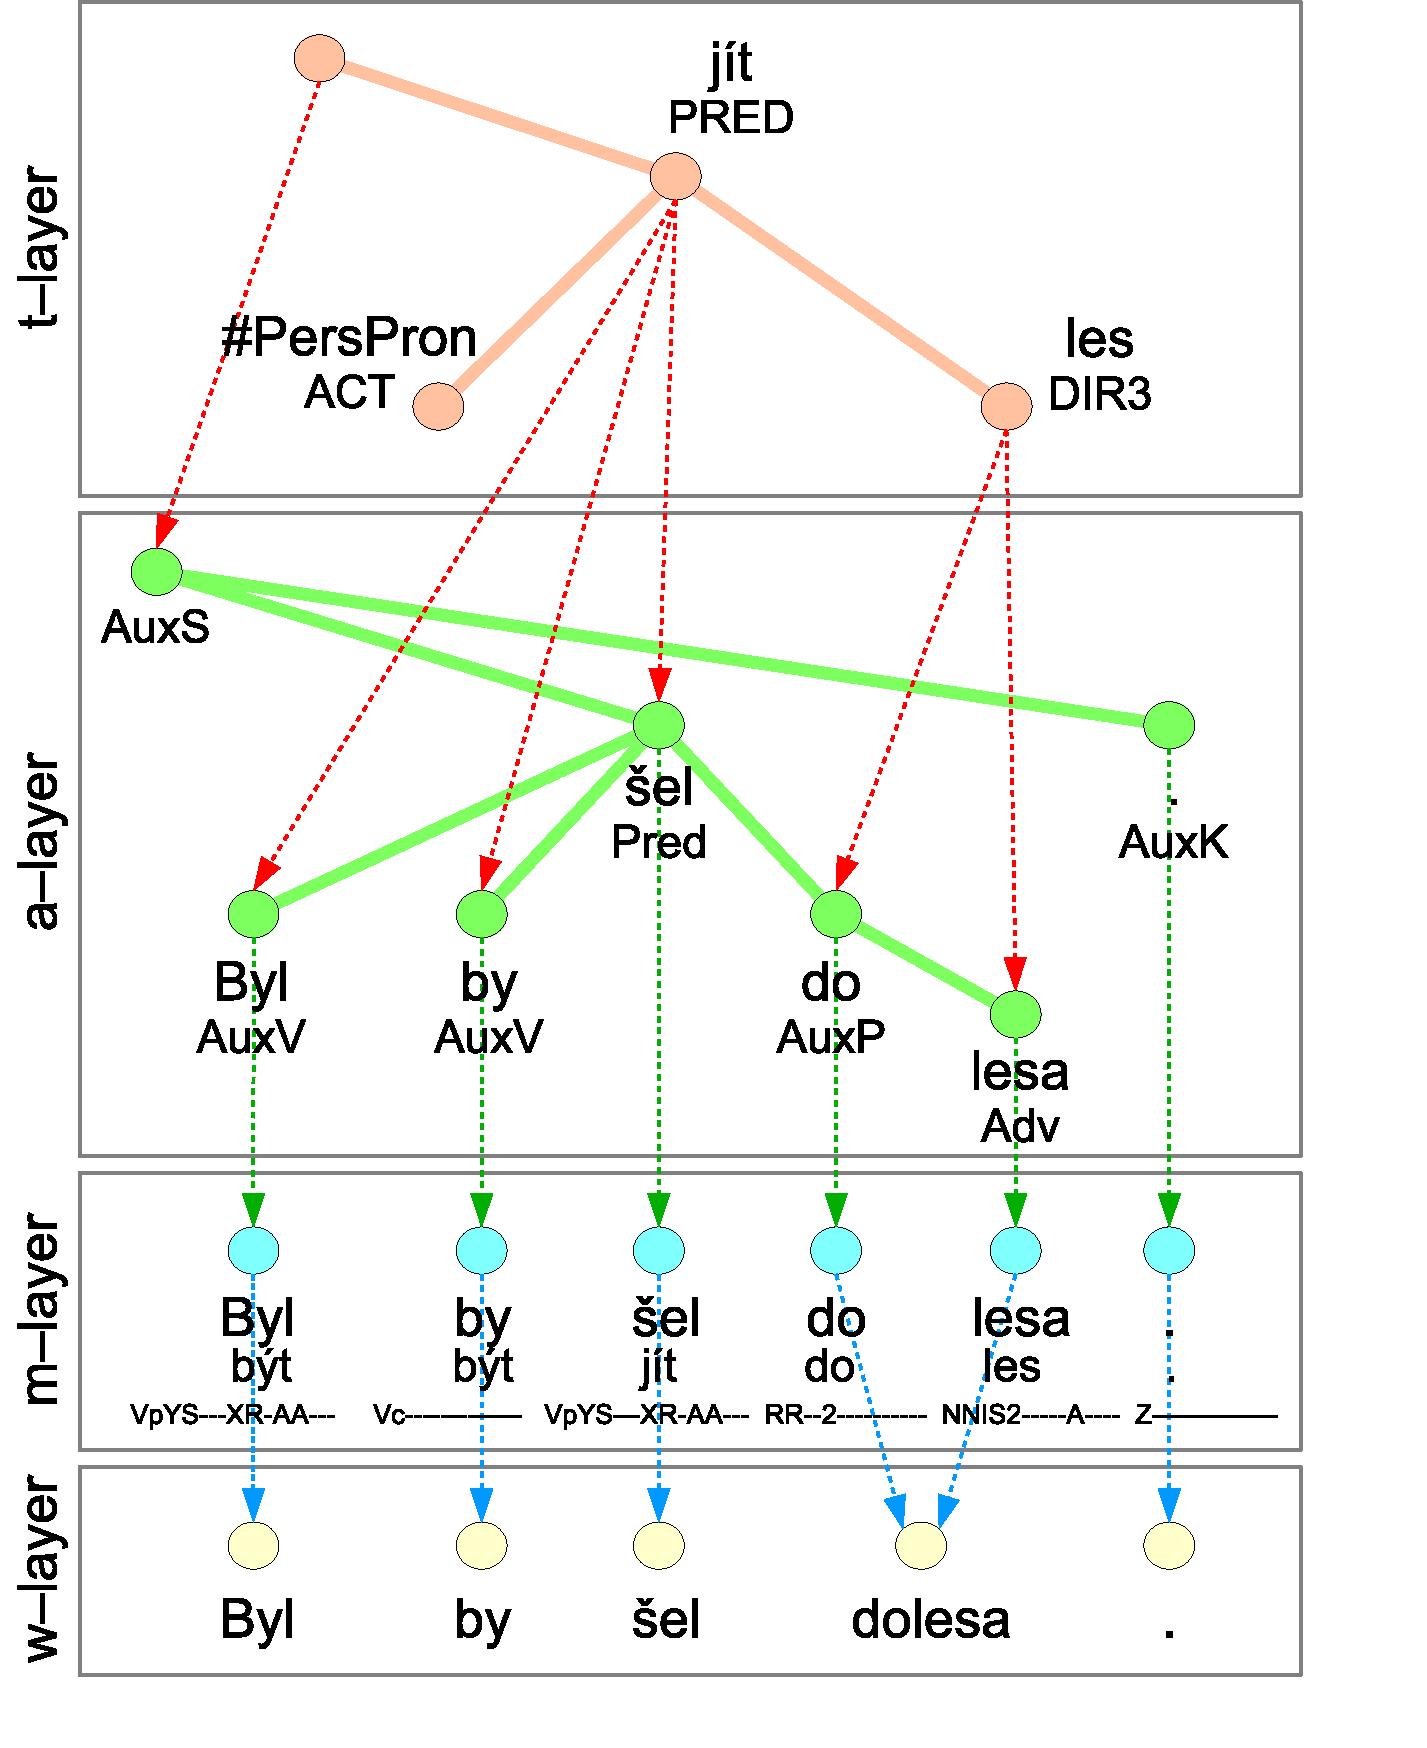
\includegraphics[height=0.9\vsize]{img/PDT_layers}
\column{.5\textwidth}
\begin{itemize}
	\item Tectogrammatical layer\\``is supposed to represent the \alert{semantic structure of a sentence}''
	\item Analytical layer (syntax)
	\item Morphological layer
\end{itemize}
\begin{itemize}
	\item PDT 2.0 on-line:\\\centerline{\scriptsize\url{http://ufal.mff.cuni.cz/pdt2.0/}} 
\end{itemize}
\vspace{0.8cm}
\emph{Sentence:}
\medskip
\\Byl by �el dolesa.
\\He-was would went toforest.
\end{columns}
\end{frame}

\begin{frame}{Tools for machine linguistic annotation}
	\begin{enumerate}
		\item Segmentation and tokenization
		\item Morphological analysis
		\item Morphological tagging	
		\item McDonnald's Maximum Spanning Tree parser\\ -- Czech adaptation
		\item Analytical function assignment
		\item Tectogrammatical analysis\\	-- Developed by V�clav Klime�
	\end{enumerate} 
	\begin{itemize}
		\item Available within the \alert{TectoMT}\footnote{\url{http://ufal.mff.cuni.cz/tectomt/}} project
	\end{itemize}
\end{frame}

\begin{frame}{Example of tectogrammatical tree}
\begin{columns}
\column{.5\textwidth}
\includegraphics[height=0.9\vsize]{img/DedVoj_tecto_tree}
\column{.5\textwidth}
\begin{itemize}
	\item Lemmas
	\item Functors
	\item Semantic parts of speech
\end{itemize}
\vspace{0.7cm}
\emph{Sentence:}
\medskip
{\small
\\Ve zdemolovan�m trabantu na m�st� zem�eli dva mu�i -- 82let� senior a dal�� mu�, jeho� toto�nost zji��uj� policist�.
\medskip
\\Two men died on the spot in demolished trabant -- \dots }
\end{columns}
\end{frame}


\subsection{Overview of the present work}


\begin{frame}{Introduction to the Presented Work}
\begin{itemize}
	\item Extraction of semantic information from \alert{texts}.	
		\begin{itemize}
			\item In Czech language.
			\item Coming from web pages.
		\end{itemize}
%	\item Using of Semantic Web \alert{ontologies}.
%		\begin{itemize}
%			\item RDF, OWL
%		\end{itemize}
	\item Exploiting of linguistic tools.
		\begin{itemize}
			\item \textbf{Prague Dependency Treebank} project.
			\item \textbf{TectoMT} project (�FAL MFF UK).
			\item \textbf{GATE} project (The University of Sheffield).
			\item Experiments with the \textbf{Czech WordNet}.
		\end{itemize}
	\item \alert{Rule based} extraction method.
		\begin{itemize}
			\item Extraction rules $\approx$ linguistic \alert{tree queries}
			\item \alert{ILP learning} of extraction rules
		\end{itemize}
\end{itemize}
\end{frame}

%\begin{frame}{Schema of the extraction process}
%\begin{columns}
%\column{.3\textwidth}
%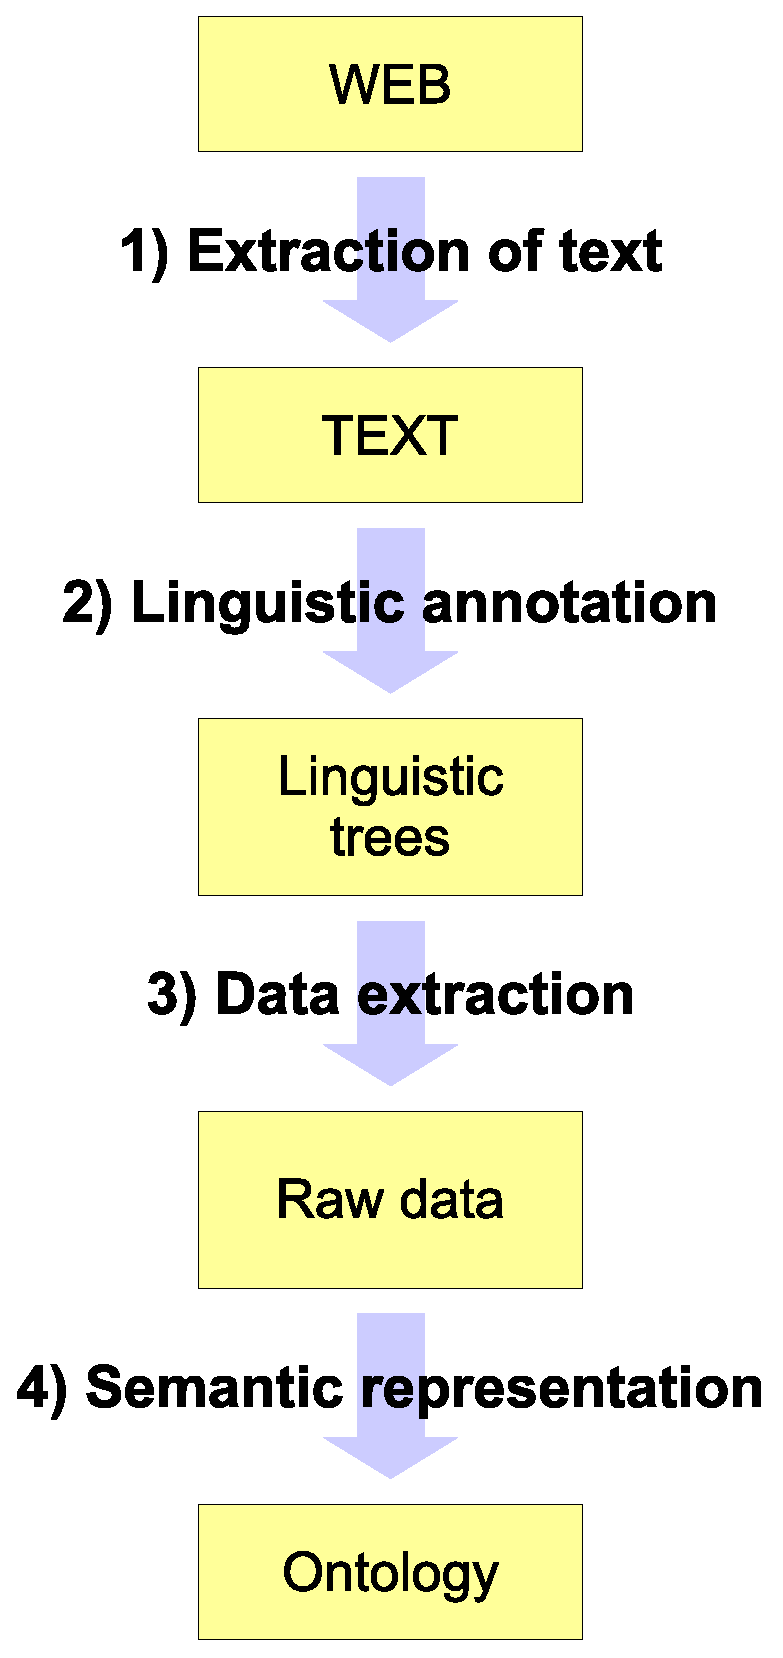
\includegraphics[height=0.8\vsize]{img/AP_schema1_en}
%\column{.7\textwidth}
%\begin{enumerate}
%\item Extraction of text
%\bigskip
%%\begin{itemize}
%%	\item Using \alert{RSS feed} to download pages.
%%	\item \alert{Regular expression} to extract text.
%%\end{itemize}
%\item Linguistic annotation
%\bigskip
%%\begin{itemize}
%%	\item Using \alert{chain} of 6 linguistic tools\\(see on next slides).
%%\end{itemize}
%%In this phase the linguistic annotators process the extracted text and produce corresponding set of dependency trees representing the deep syntactic structure of individual sentences. We have used the linguistic tools described in the section~\ref{sec:ling_tools} for this task.
%\item \alert{Data/Information extraction}
%\bigskip
%%\begin{itemize}
%%	\item Exploitation of linguistic trees.
%%	\item Using \alert{extraction rules}.	
%%\end{itemize}
%%We use the structure of tectogrammatic (i.e. deep syntactic) dependency trees to extract relevant data. 
%\item Semantic representation of data
%\bigskip
%%\begin{itemize}
%%	\item Ontology needed.
%%	\item Semantic interpretation of rules.
%%	\item Far from finished in current state.
%%\end{itemize}
%%This phase consists of quite simple data transformation or conversion to the desired ontology format. But it is quite important to choose suitable ontology that will properly represent semantics of the data. We have not implemented this phase yet.
%\end{enumerate}
%\end{columns}
%\end{frame}
%
%
%\begin{frame}{Domain of our experiments}
%\begin{itemize}
%	\item \alert{Fire-department articles}
%	\item From The Ministry of Interior of the Czech Republic\footnote{\url{http://www.mvcr.cz/rss/regionhzs.html}}
%	\item Extensive experiments
%		\begin{itemize}
%			\item More than 800 articles 
%			%\\from different regions of Czech Republic
%			\item 1.2 MB of textual data
%%			\item Linguistic tools produced 10 MB of annotations,\\run time 3.5 hours
%			\item Extracting information about injured and killed people
%			\item 470 matches of the extraction rule,\\200 numeric values of quantity (described later)
%		\end{itemize}
%	\item \alert{Intensive experiments}	
%		\begin{itemize}
%			\item 50 articles
%			\item Precisely manually tagged
%			\item Used of the evaluation of the learning procedure
%		\end{itemize}
%\end{itemize}
%\end{frame}
%
%\begin{frame}{Example of the web-page with a report of a fire department}
%\begin{columns}
%\column{\textwidth}
%\includegraphics[height=0.9\vsize]{img/DedVoj_article}
%\end{columns}
%\end{frame}
%


\begin{frame}{Example of processed text -- a fire accident}
\centerline{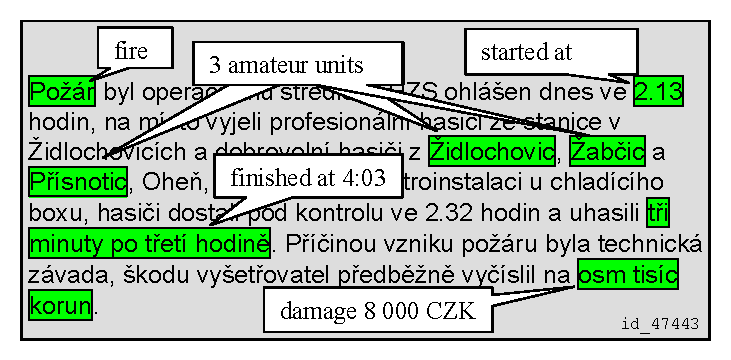
\includegraphics[height=0.5\vsize]{img/message}}
\bigskip
\begin{itemize}
	\item Information to be extracted is decorated.
	\item See the last sentence on the \alert{next slide}.
\end{itemize}
\end{frame}

\begin{frame}{Example of a linguistic tree}
\centerline{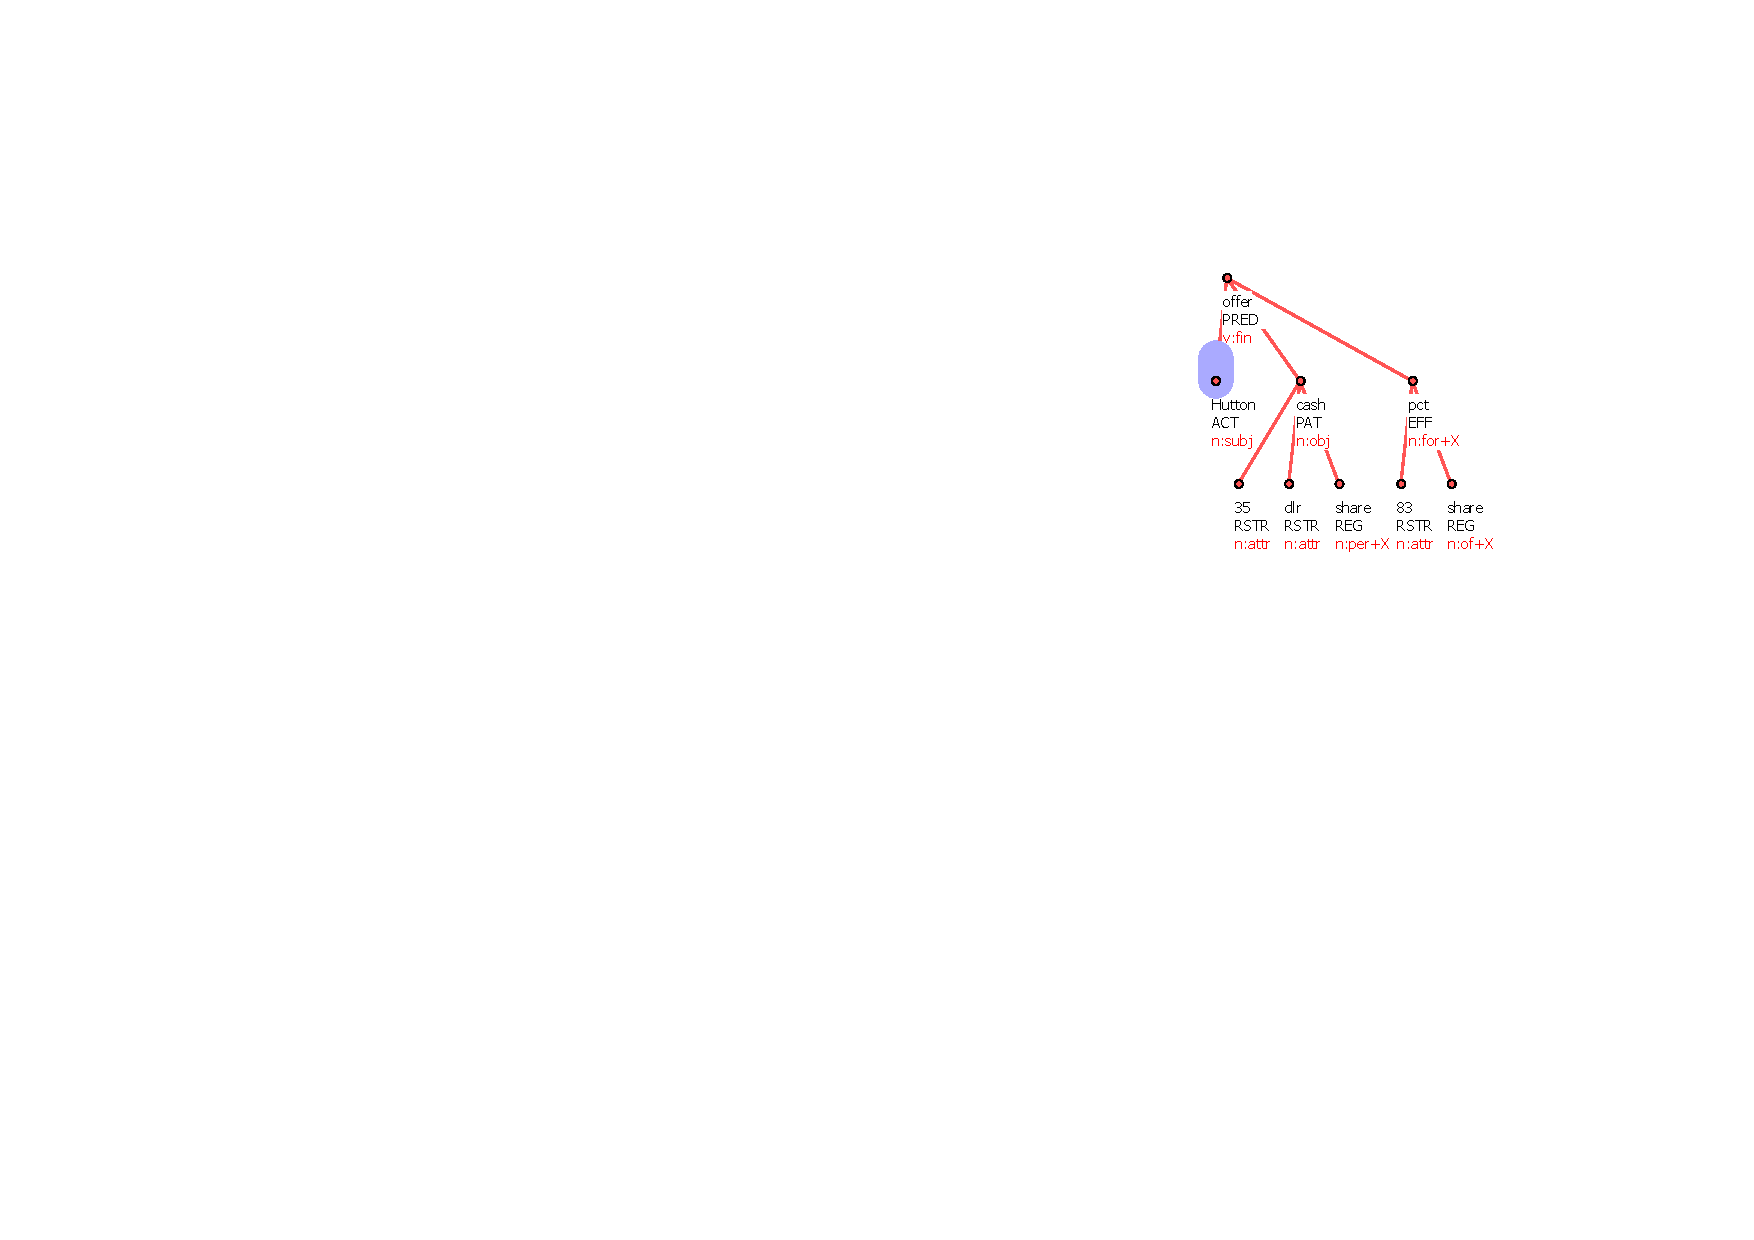
\includegraphics[height=0.7\vsize]{img/tree}}
\begin{itemize}
	\item Our IE method uses \alert{tree queries} (tree patterns)
\end{itemize}
\end{frame}



\section{Our Information Extraction Method}


\subsection{Manually created rules}

\frame{\tableofcontents[currentsubsection]}
%\begin{frame}[plain]
%\begin{columns}
%\column{.67\textwidth}
%%\centerline{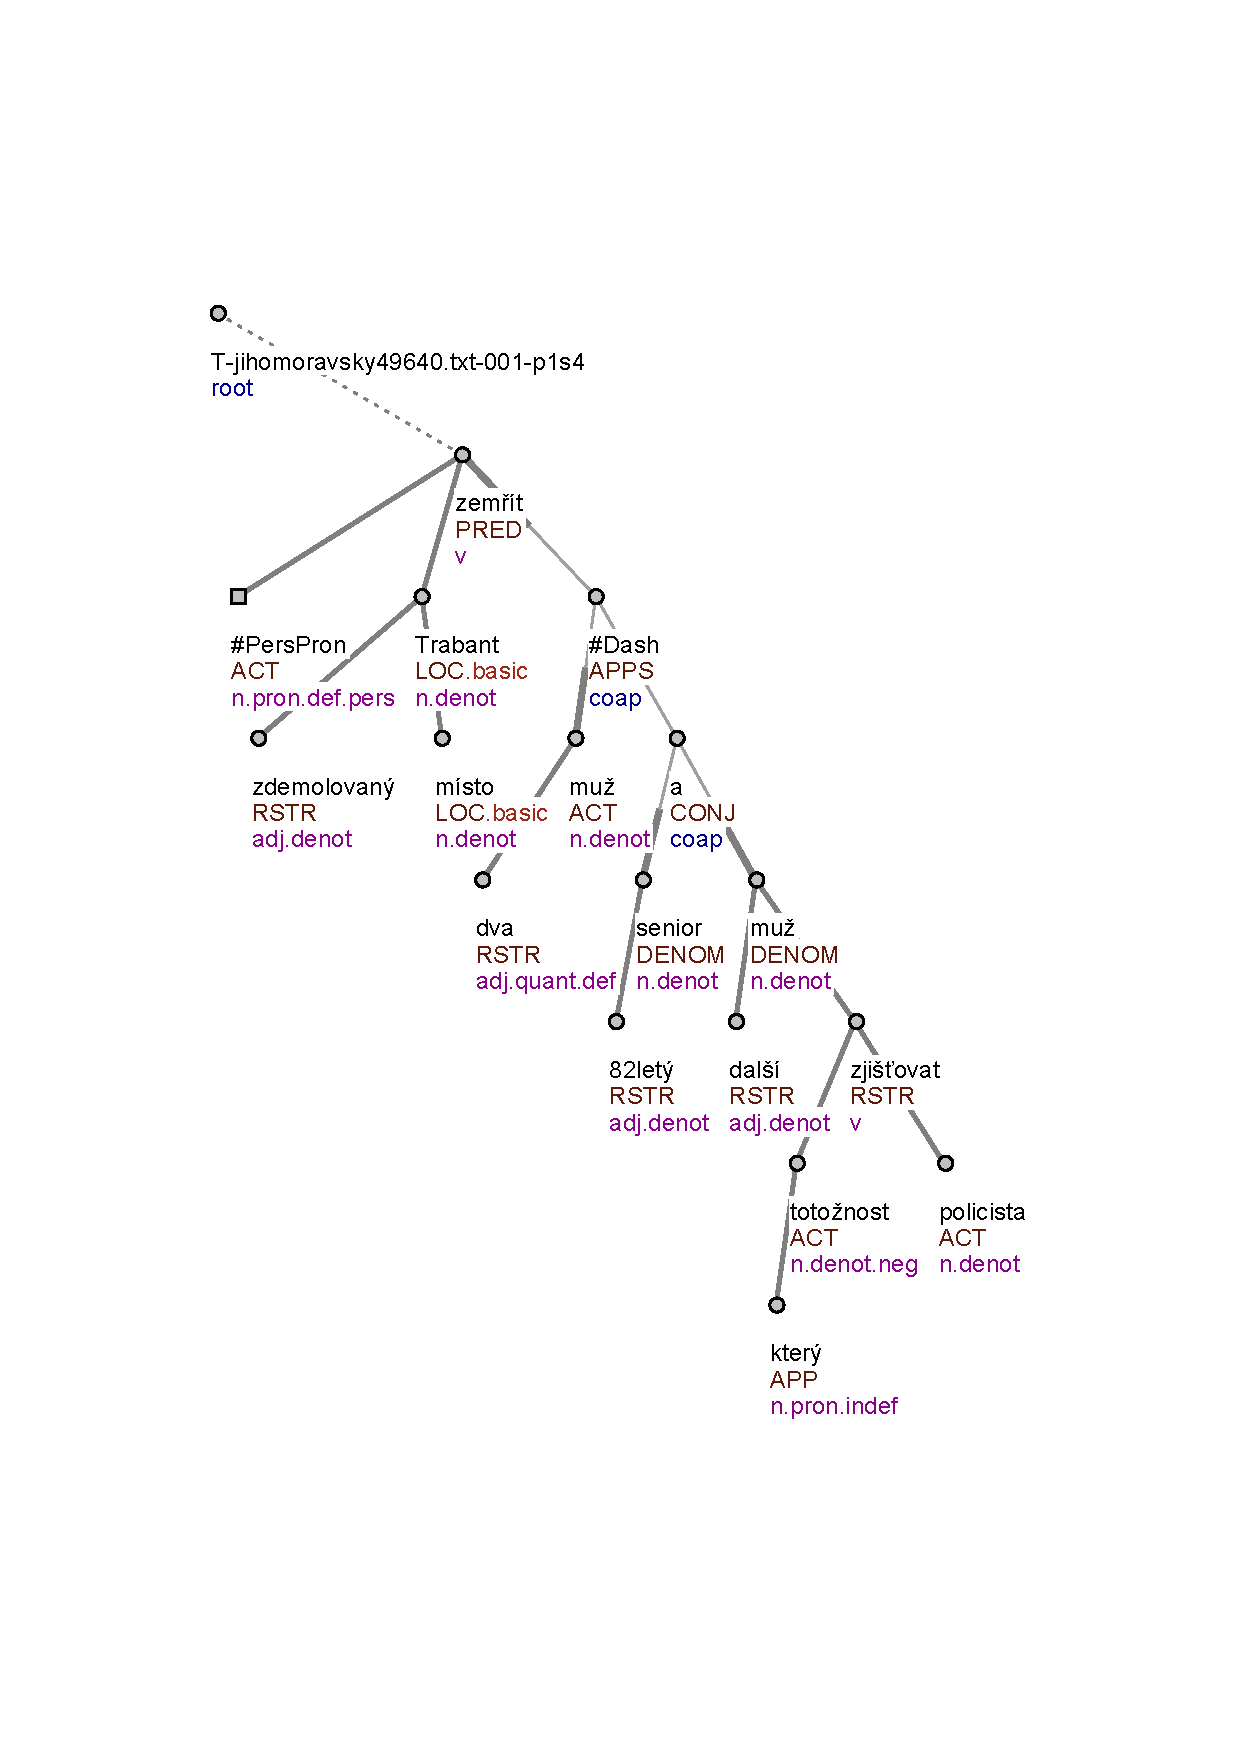
\includegraphics[height=1.1\vsize,width=\hsize]{img/TectogramaticalTree}}
%\centerline{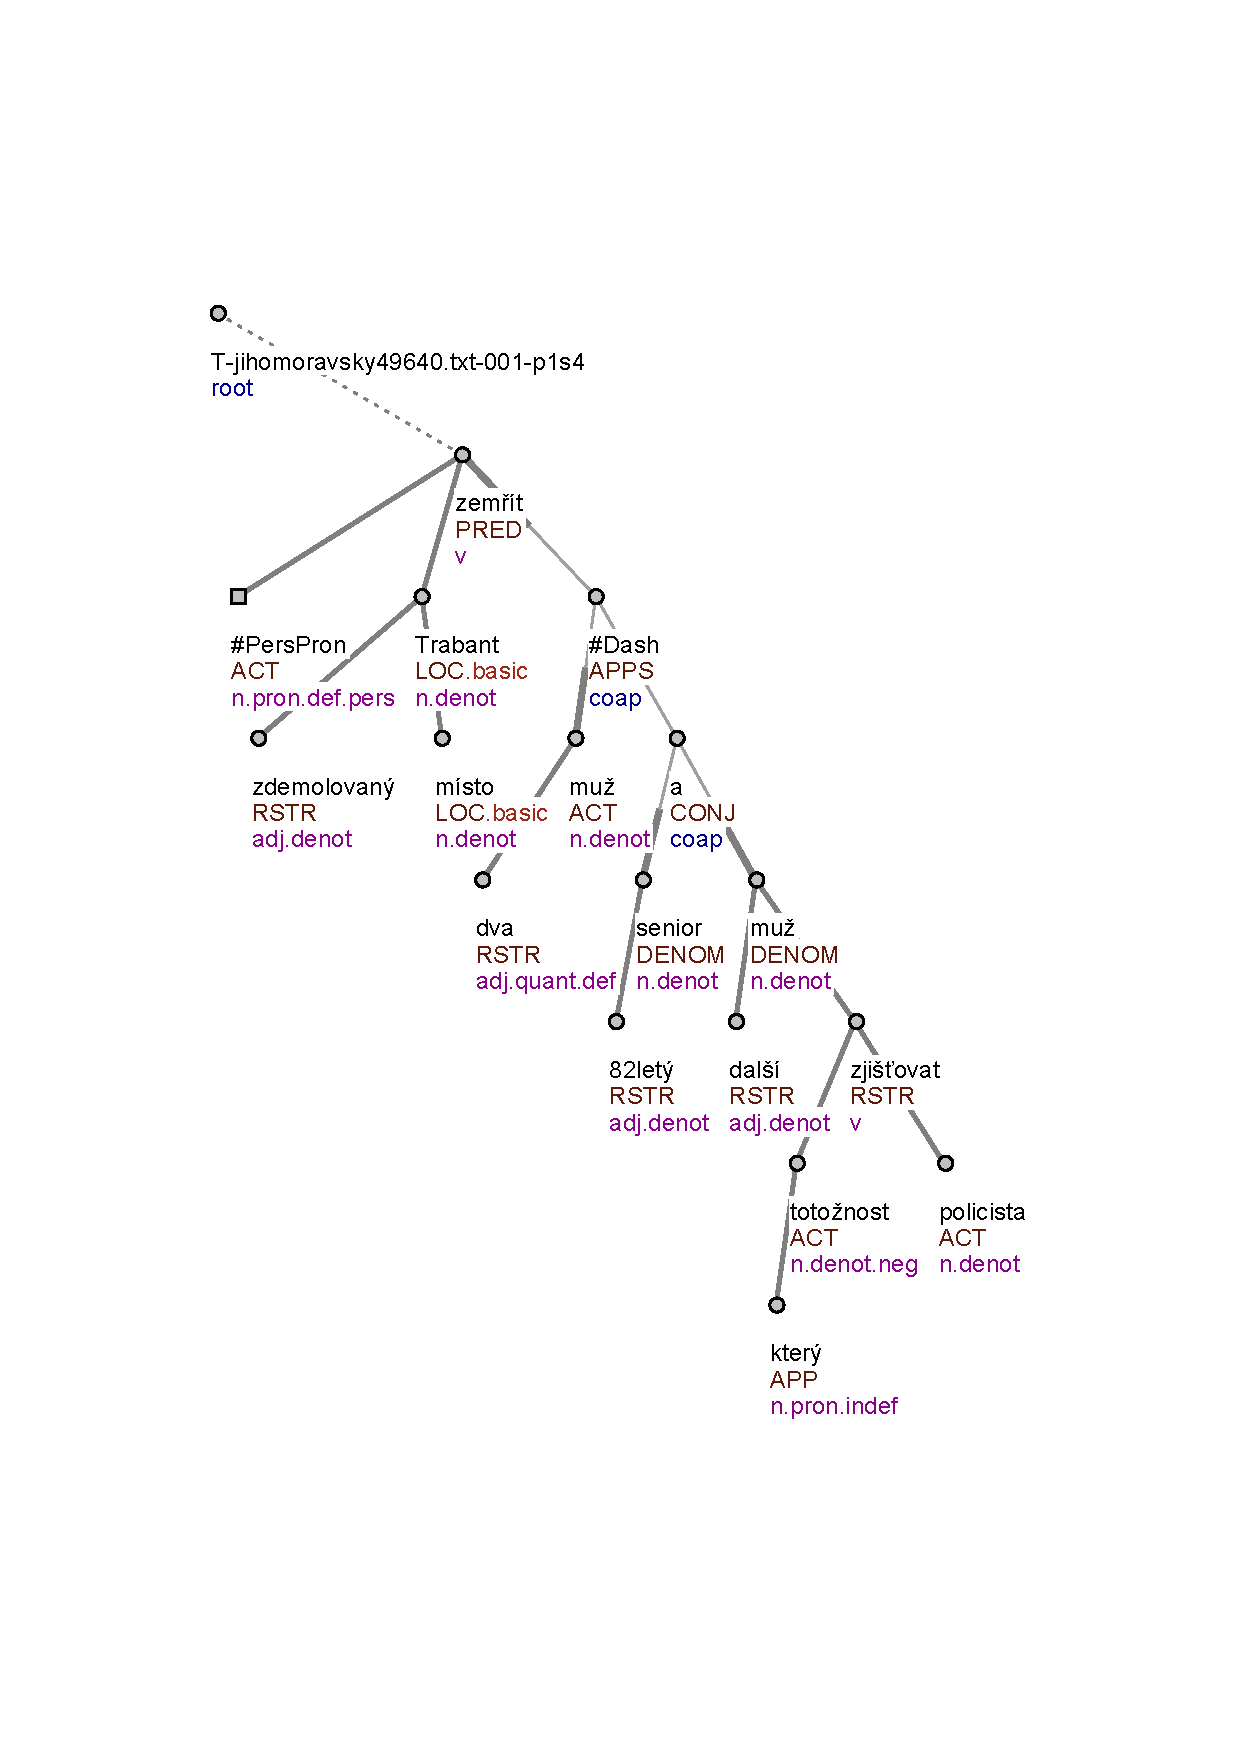
\includegraphics[height=1.1\vsize]{img/TectogramaticalTree}}
%\column{.33\textwidth}
%\begin{itemize}
%	\item How to extract the information about \alert{two dead} people?
%\end{itemize}
%\vspace{2cm}
%\end{columns}
%\end{frame}

\begin{frame}{Extraction rules -- Netgraph queries}
\begin{center}
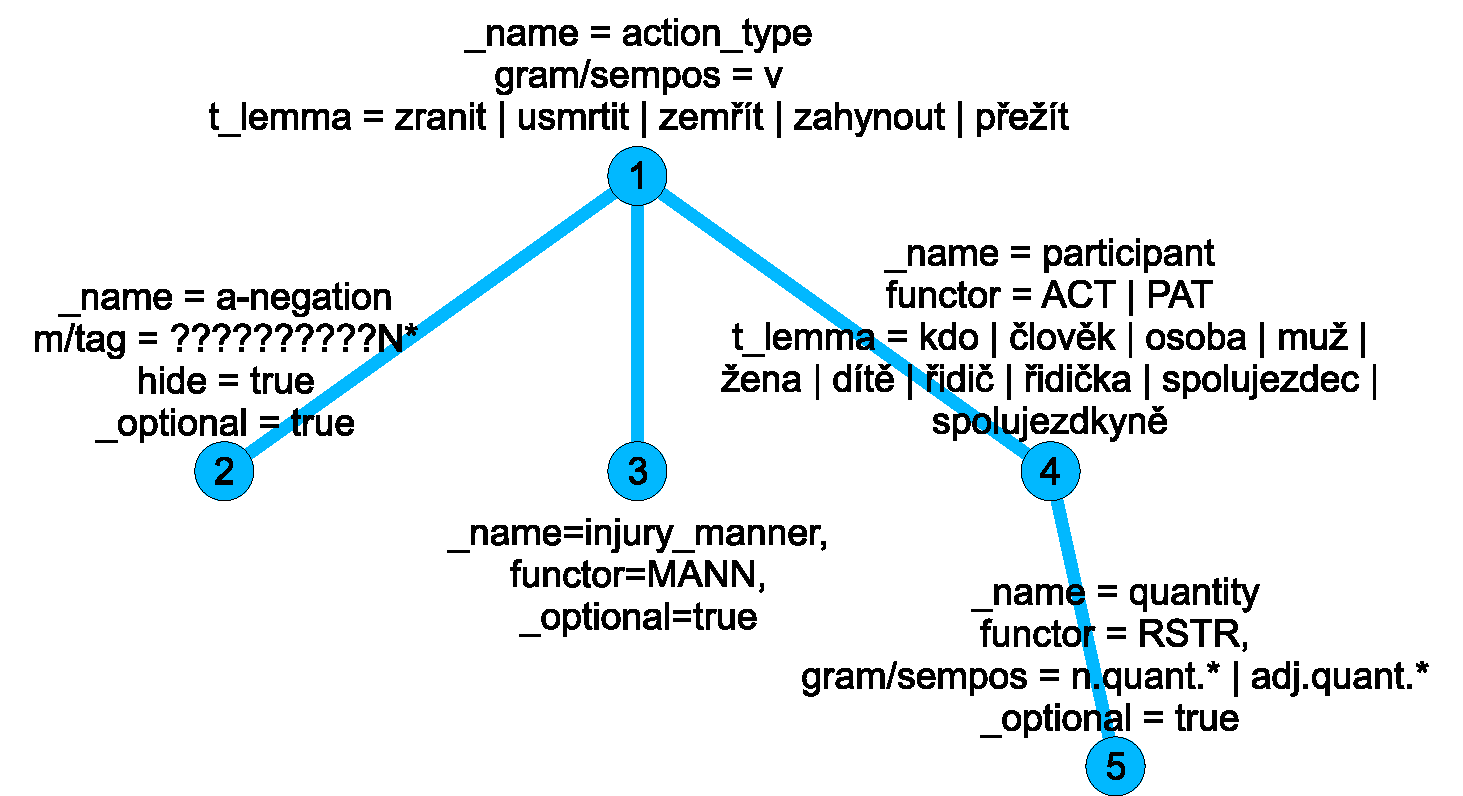
\includegraphics[height=0.6\vsize]{img/extract_patern}
\end{center}
\begin{itemize}
	\item Tree patterns on \alert{shape} and \alert{nodes} (on node attributes).
	\item Evaluation gives \alert{actual matches} of particular nodes.
	\item \alert{Names} of nodes allow use of references.
\end{itemize}
\end{frame}


\begin{frame}{Raw data extraction output}
%\begin{center}
\centerline{\includegraphics[height=0.8\vsize]{img/DedVoj_OutputQueryMatches}}
%\end{center}

{\scriptsize
\textbf{SELECT} \alert{action\_type}.t\_lemma, \alert{a-negation}.m\/tag, 
\alert{injury\_manner}.t\_lemma, \alert{participant}.t\_lemma,
\alert{quantity}.t\_lemma \textbf{FROM} \emph{***extraction rule***} 
}
\end{frame}


\begin{frame}{Semantic interpretation of extraction rules}
\begin{center}
\includegraphics[width=\hsize]{img/DedVoj_semantic_interpretation}
\end{center}
\begin{itemize}
	\item Determines how particular values of attributes are used.
	\item Gives semantics to extraction rule.
	\item Gives semantics to extracted data.
\end{itemize}
\end{frame}

%\begin{frame}{Semantic data output}
%\includegraphics[width=\hsize]{img/DedVoj_instances}
%\bigskip
%\begin{itemize}
%	\item Two instances of two ontology classes.
%\end{itemize}
%\end{frame}
%
%
%\begin{frame}{The experimental ontology}
%\begin{columns}
%\column{.45\textwidth}
%\includegraphics[height=0.6\vsize]{img/DedVoj_classes}
%\column{.55\textwidth}
%\begin{itemize}
%	\item Two \alert{classes}	
%		\begin{itemize}
%			\item Incident and Participant
%		\end{itemize}
%	\item One \alert{object property} relation
%		\begin{itemize}
%			\item hasParticipant
%		\end{itemize}
%	\item Five \alert{datatype property} relations
%		\begin{itemize}
%			\item actionManner \\(light or heavy injury)
%			\item negation
%			\item actionType \\(injury or death)
%			\item participantType \\(man, woman, driver, etc.)
%			\item participantQuantity
%		\end{itemize}
%\end{itemize}
%\end{columns}
%\end{frame}

%\begin{frame}{Design of extraction rules -- iterative process}
%\begin{center}
%\includegraphics[height=0.6\vsize]{img/DedVoj_coverge_tuning}
%\end{center}
%\begin{enumerate}
%	\item \alert{Frequency analysis} $\rightarrow$ representative key-words.
%	\item Investigating of matching trees $\rightarrow$ \alert{tuning} of tree query.
%	\item \alert{Complexity} of the query $\cong$ complexity of extracted data.
%\end{enumerate}
%\end{frame}



\subsection{Learning of rules}
\frame{\tableofcontents[currentsubsection]}

\begin{frame}{Integration of ILP in our extraction process}
\begin{center}
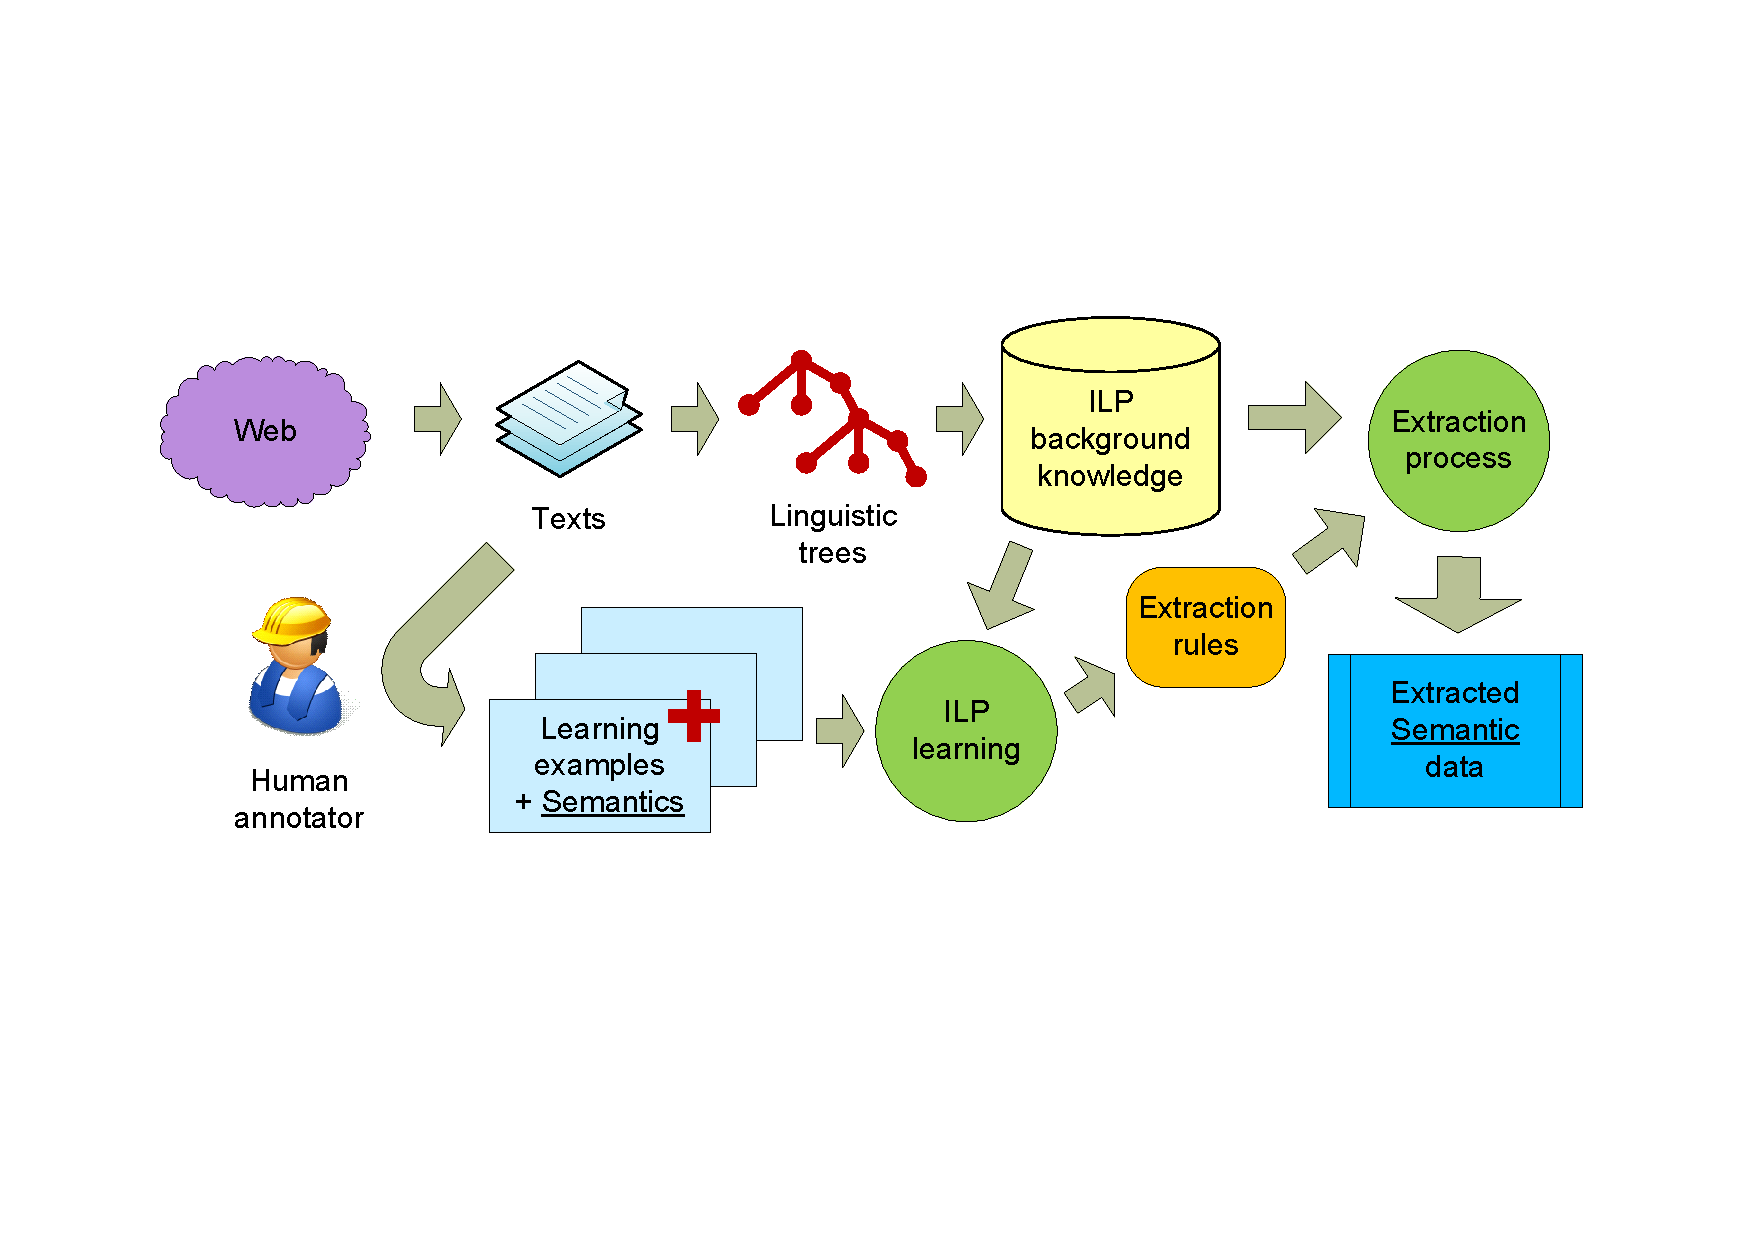
\includegraphics[width=\hsize]{img/DedVoj_ILP}
\end{center}
\begin{itemize}
	\item Transformation of trees to \alert{logic representation}. 
\end{itemize}
\end{frame}

\begin{frame}{Logic representation of linguistic trees}
\begin{columns}
\column{\textwidth}
\includegraphics[height=0.9\vsize]{img/DedVoj_LogicRepresentation}
\end{columns}
\end{frame}

\begin{frame}{Root/Subtree Preprocessing/Postprocessing (Chunk learning)}
\centerline{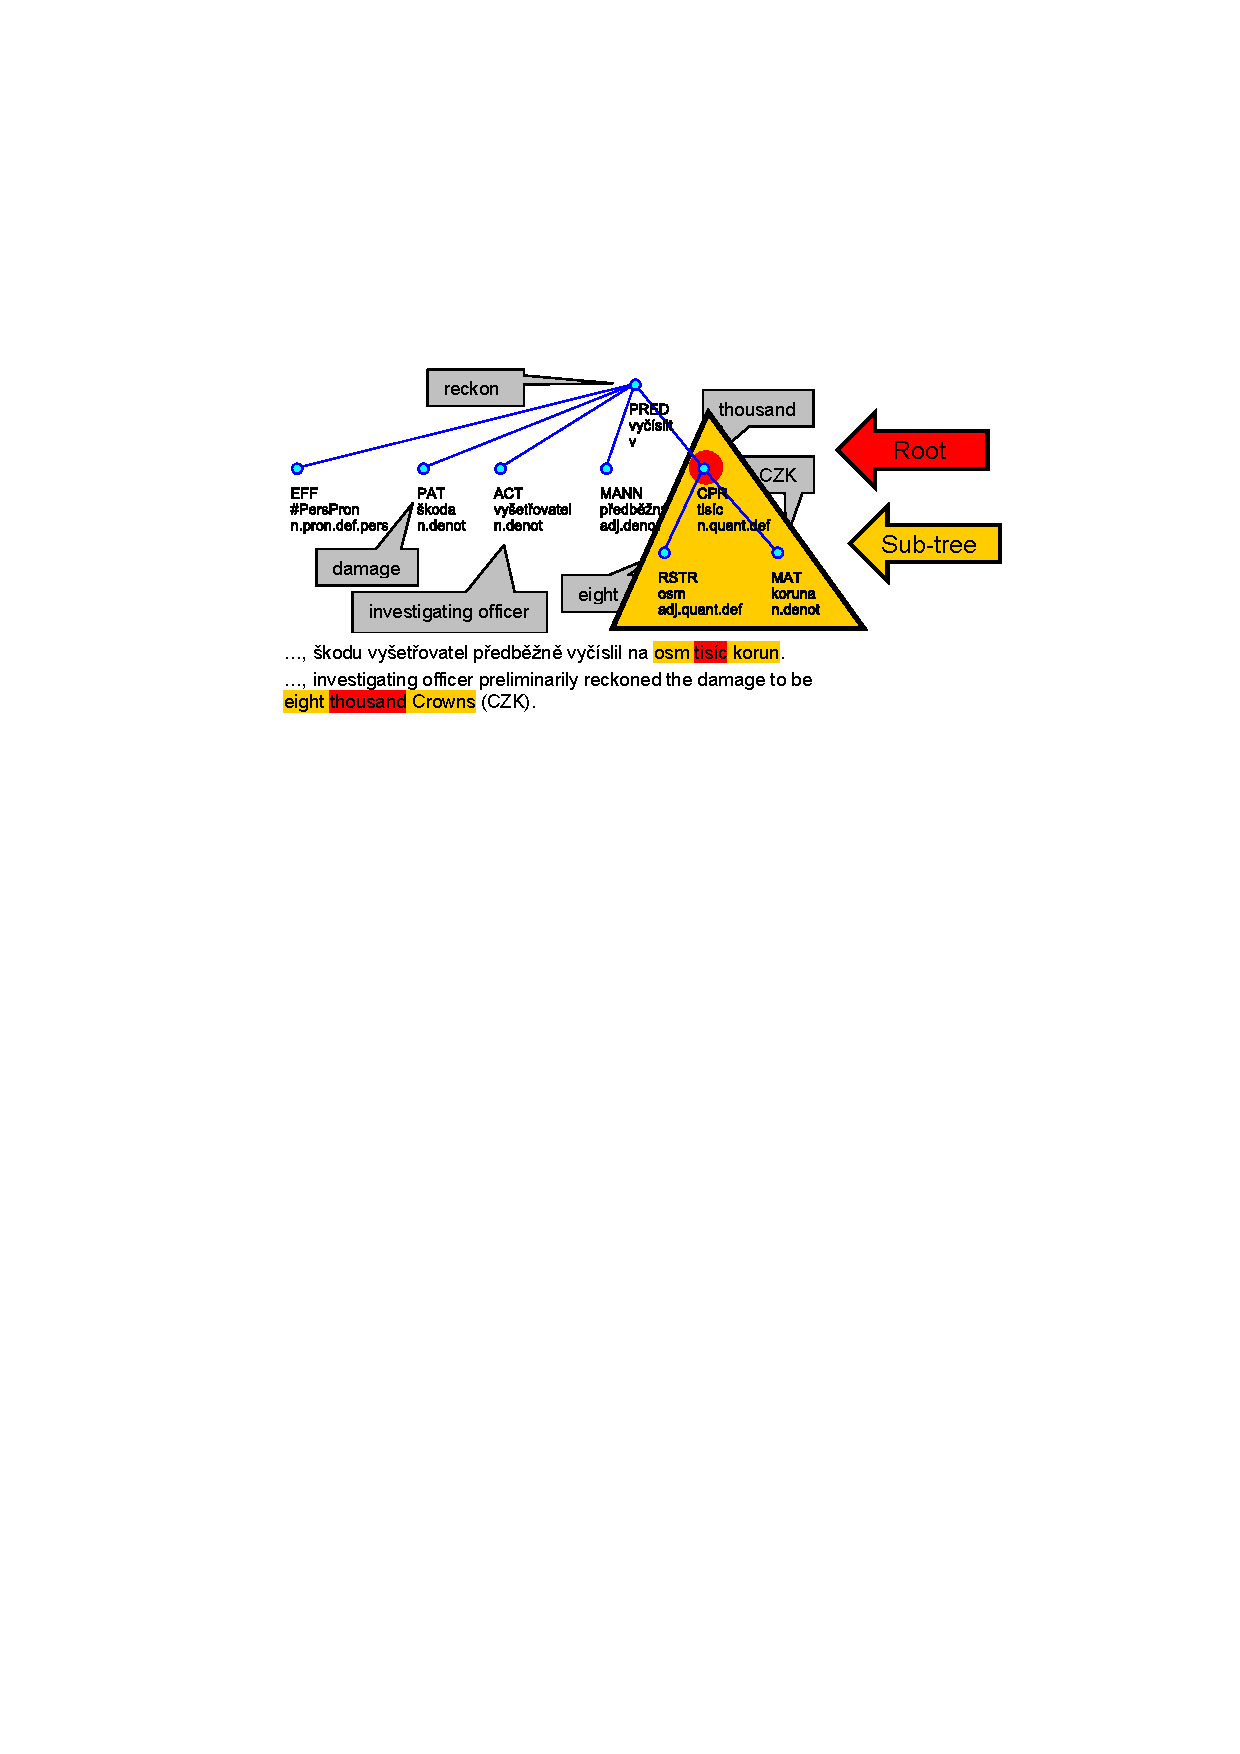
\includegraphics[width=\hsize]{img/tree-subtree}}
\end{frame}


\begin{frame}[fragile]{Examples of learned rules, Czech words are translated.}
\begin{example}
{\scriptsize


[Rule 1] [Pos cover = 14 Neg cover = 0]\\
\verb@damage_root(A) :- lex_rf(B,A), has_sempos(B,'n.quant.def'),@
\verb@   tDependency(C,B), tDependency(C,D),@ 
\verb@   has_t_lemma(D,'investigator').@ %\emph{\%vy353et345ovatel = investigator}
\smallskip

[Rule 2] [Pos cover = 13 Neg cover = 0]\\
\verb@damage_root(A) :- lex_rf(B,A), has_functor(B,'TOWH'),@
\verb@   tDependency(C,B), tDependency(C,D), has_t_lemma(D,'damage').@\\
\bigskip


[Rule 1] [Pos cover = 7 Neg cover = 0]\\
\verb@injuries(A) :- lex_rf(B,A), has_functor(B,'PAT'),@
\verb@   has_gender(B,anim), tDependency(B,C), has_t_lemma(C,'injured').@\\
\smallskip

[Rule 8] [Pos cover = 6 Neg cover = 0]\\
\verb@injuries(A) :- lex_rf(B,A), has_gender(B,anim), tDependency(C,B),@
\verb@   has_t_lemma(C,'injure'), has_negation(C,neg0).@

}
%{\tiny \begin{verbatim}
%contains_num_injured(A) :- t_lemma(A,1).
%contains_num_injured(A) :- t_lemma(A,2).
%contains_num_injured(A) :- t_lemma(A,23).
%contains_num_injured(A) :- edge(A,B), m_form(B,jeden).
%contains_num_injured(A) :- edge(A,B), m_tag(B,cn_s1__________).
%contains_num_injured(A) :- edge(B,A), functor(B,conj).
%contains_num_injured(A) :- edge(B,A), t_lemma(B,dite).
%contains_num_injured(A) :- edge(B,A), t_lemma(B,muz).
%contains_num_injured(A) :- edge(B,A), edge(B,C), m_tag14(C,1).
%contains_num_injured(A) :- edge(B,A), edge(B,C), t_lemma(C,tezky).
%contains_num_injured(A) :- edge(B,A), edge(B,C), t_lemma(C,nasledek).
%contains_num_injured(A) :- edge(A,B), edge(C,A), m_tag4(B,1), functor(C,pat).
%contains_num_injured(A) :- edge(A,B), edge(C,A), functor(C,act), a_afun(B,sb).
%contains_num_injured(A) :- edge(B,A), edge(C,B), edge(C,D), t_lemma(D,vloni).
%contains_num_injured(A) :- edge(B,A), edge(C,B), t_lemma(B,osoba), t_lemma(C,zranit).
%contains_num_injured(A) :- edge(B,A), edge(C,B), t_lemma(B,osoba), t_lemma(C,zemrit).
%contains_num_injured(A) :- edge(B,A), edge(C,B), functor(B,act), edge(C,D),
%                           a_afun(D,obj).
%contains_num_injured(A) :- edge(B,A), edge(C,B), t_lemma(B,osoba), edge(C,D), edge(D,E),
%                           functor(D,twhen).
%contains_num_injured(A) :- edge(B,A), t_lemma(A,tri), edge(B,C), edge(D,B), edge(E,D),
%                           m_tag2(C,m).
%\end{verbatim}}
\end{example}
\end{frame}



\subsection{Evaluation}
\frame{\tableofcontents[currentsubsection]}


\begin{frame}{Evaluation results}

\centerline{
\scriptsize
\begin{tabular}{|l||r|r|r|r|r|r|r|}
\hline
\textbf{task/method} & \textbf{matching} & \textbf{missing} & \textbf{excess} & \textbf{overlap} & \textbf{prec.}\% & \textbf{recall}\% & \textbf{F1.0}\%\\
\hline
\hline
\textbf{damage/ILP} & 14 & 0 & 7 & 6 & 51.85 & 70.00 & 59.57\\
\hline
\multicolumn{5}{|l|}{\textbf{damage/ILP -- lenient measures}} & 74.07 & 100.00 & 85.11\\
\hline
\textbf{dam./ILP-roots} & 16 & 4 & 2 & 0 & 88.89 & 80.00 & \textbf{84.21}\\
\hline
\emph{\textbf{damage/Paum}} & \emph{20} & \emph{0} & \emph{6} & \emph{0} & \emph{76.92} & \emph{100.00} & \emph{86.96}\\
\hline
\hline
\textbf{injuries/ILP} & 15 & 18 & 11 & 0 & 57.69 & 45.45 & \textbf{50.85}\\
\hline
\emph{\textbf{injuries/Paum}} & \emph{25} & \emph{8} & \emph{54} & \emph{0} & \emph{31.65} & \emph{75.76} & \emph{44.64}\\
\hline
\emph{\textbf{inj./Paum-afun}} & \emph{24} & \emph{9} & \emph{38} & \emph{0} & \emph{38.71} & \emph{72.73} & \emph{50.53}\\
\hline
\end{tabular}
}

\bigskip

\begin{itemize}
	\item 10-fold cross validation
	\item Two tasks: `damage' and `injuries'
	\item Root/subtree preprocessing/postprocessing used for `damage' task
\end{itemize}
\end{frame}


\section{Conclusion}
\frame{\tableofcontents[currentsection]}

\subsection{Summary}

\begin{frame}{Summary}
 \begin{itemize}
  \item Implemented a system for extraction of semantic information 
  \item Based on third party linguistic tools (\alert{TectoMT}\footnote{\url{http://ufal.mff.cuni.cz/tectomt/}})
  \item Extraction rules adopted from \alert{Netgraph}\footnote{\url{http://quest.ms.mff.cuni.cz/netgraph/}} application.
  \item \alert{ILP} used for learning rules.
  \item All methods integrated inside \alert{GATE}\footnote{\url{http://gate.ac.uk/}}.
  \bigskip
  \item Main advantages:  
	\begin{itemize}
		\item Automated selection of learning features
		\item ``Language independent''
		\item Rule based
	\end{itemize}
 \end{itemize}
\end{frame}


\subsection{Future work}

\begin{frame}{Future work}
 \begin{itemize}
			\item Use some \alert{Knowledge Base} (e.g. WordNet).
			\item Adaptation of this method on \alert{other languages}.
			\item Evaluation of the method on \alert{other datasets}.
			\item Be able to provide \alert{more semantics}.			
			\begin{itemize}
				\item e.g. sophisticated semantic interpretation of extracted data
			\end{itemize}
 \end{itemize}
\end{frame}

%\subsection{Inter-project cooperation}
%\begin{frame}{Inter-project cooperation}
% \begin{itemize}
%  \item Mainly with \textbf{I-3 Matematick� lingvistika} group
%  \item \alert{Directly} with David Mare�ek
%  \item \alert{Indirectly} with all participants of the linguistic projects
%
%\bigskip
%
%  \item Making all the linguistic tools working, updates
%  \item Planned feedback in the future \\(\alert{comparison} of linguistic tools)
%  \item \alert{Porting} PDT formalism and TMT tools to the GATE platform (side effect of our work, but may be usefull in the future).
% \end{itemize}
%\end{frame}


% no key words


\end{document}



%%% Local Variables: 
%%% mode: latex
%%% TeX-master: t
%%% End: 
